\documentclass[../lecture-notes.tex]{subfiles}

\begin{document}

\subsection{Introduction}
\textbf{Error-correcting codes (ECC)} are a group of protocols that wrap the input data extending it with an excessive 
information that allows recovery of the original data even if the received message contains errors. Such methods are 
widely used in the network protocols and data storage approaches. Moreover, they found many applications in the modern 
cryptographic protocols (for example, Reed-Solomon ECC has been applied in the FRI protocol, which is widely used in 
ZK-STARKs). Additionally, each code allows the determination of what errors exactly appeared in the received message 
(sometimes, even if the message can not be decoded).

ECC protocols can be divided in two groups: \textbf{block codes} and \textbf{convolutional codes}. The block codes 
split information into the blocks of fixed pre-defined size and apply encoding to each block separately, while the 
convolutional codes work over the input data stream of an arbitrary size. Modern practical block codes allow encoding 
by polynomial complexity algorithms depending on the block size. Also, most of classic block codes leverage the 
properties of the finite fields.

In this article we primarily describe the structure of some classic block ECCs, including Walsh-Hadamard code and 
Reed-Solomon code. Its aim is to give the  reader an understanding of how they work and the mathematical primitives 
they rely on.

\subsection{Preliminaries}

First of all let's define the main property of each ECC that directly determines its structure:
\begin{definition}
For the arbitrary binary strings of fixed length $x, y \in \{0, 1\}^n$ we define \textbf{Hamming distance} as the 
number of elements where our binary strings do not match, divided by the length of the string: 
$\Delta(x,y) = \frac{1}{n}|\{i: x_i \neq y_i\}|$.
\end{definition}
Then, we can define what exactly a block ECC is. Basically, it operates over some field ($GF(2)$ for example) encoding 
information using some algorithm that differs for each code.
\begin{definition}
For each $\delta \in [0, 1]$ we call a function $E: \{0, 1\}^n \rightarrow \{0, 1\}^m$ an 
\textbf{error-correcting code} with distance $\delta$ if for each two input strings $x \neq y \in \{0, 1\}^n$ the 
distance between their images is more or equal $\delta$: $\Delta(E(x), E(y)) \geq \delta$. We call $Im(E)$  the set 
of \textbf{codewords} of the corresponding code.
\end{definition}
Thus, each block ECC that takes an input word of size $n$ and outputs a codeword of size $m$ can theoretically deal 
with $t = m-n$ errors. A block ECC also utilizes a relation between its distance and its theoretical correcting 
capability: $t < \lfloor \frac{d-1}{2} \rfloor$. This relation exists because two arbitrary codewords can be decoded 
if they contain at most $t$ errors. Therefore, the distance between these codewords must be at least $2t$ to enable 
unique decoding (if it is less then two different codewords with errors can be represented as the same message, so the 
pre-image cannot be found correctly). While the ECC distance is $d$, it leads to the relation above 
(check Figure \ref{fig:distance}).
\begin{figure}[H]
    \centering
    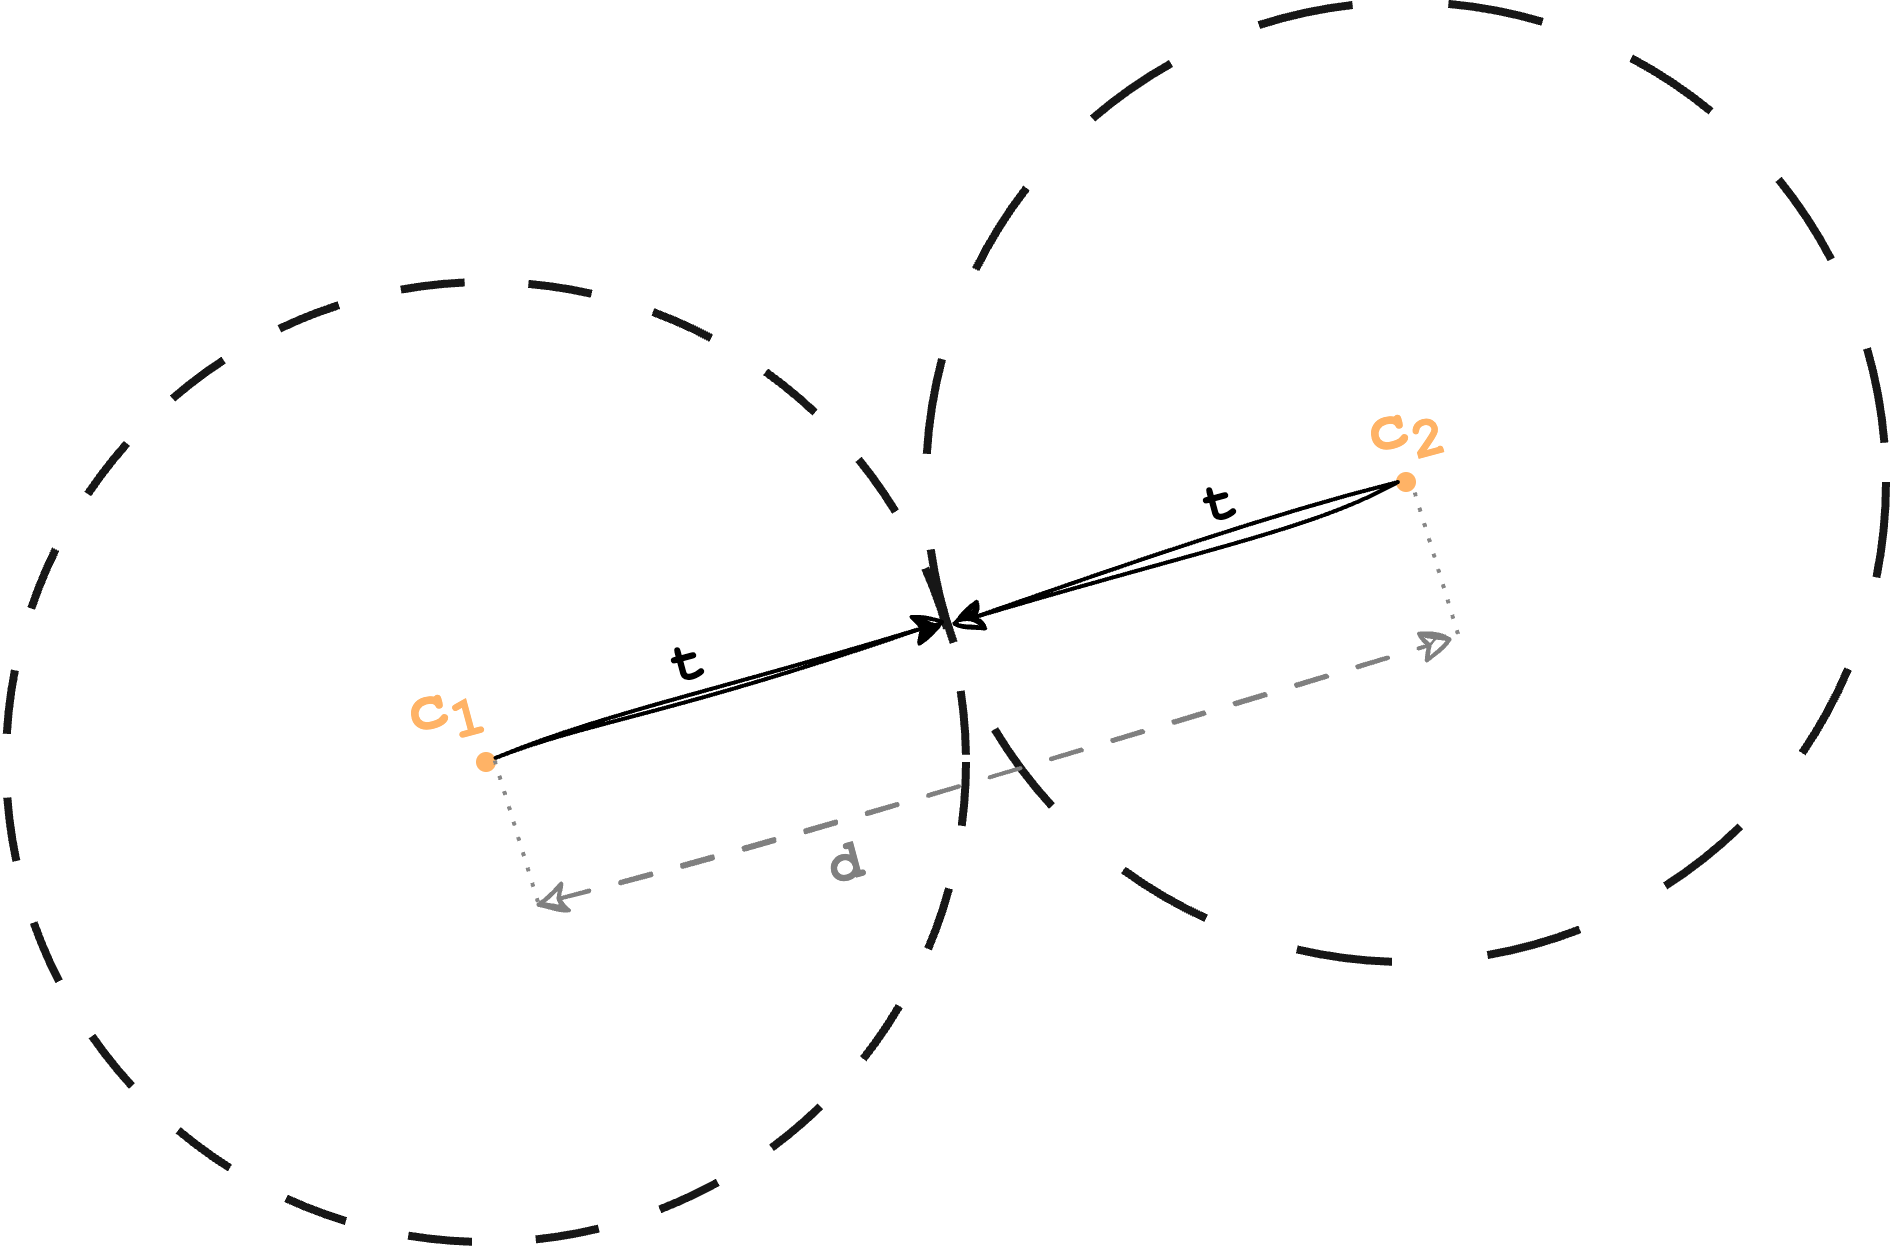
\includegraphics[width=0.5\linewidth]{images/lecture_14/circles.png}
    \caption{Relation between distance and the number of possible errors}
    \label{fig:distance}
\end{figure}

\subsection{Walsh-Hadamard code}
The Hadamard code, named after French mathematician Jacques Hadamard, is an error-correcting block code designed for 
detecting and correcting errors in message transmissions over highly noisy or unreliable channels. In 1971, NASA 
utilized this code to send images of Mars from the Mariner 9 space probe back to Earth. This code is also referred to 
as the Walsh code, Walsh family, or Walsh–Hadamard code, in honor of American mathematician Joseph Leonard Walsh.

\begin{definition}[Walsh-Hadamard code]
For the binary strings $x, y \in \{0, 1\}^n$ let's define $\langle x, y \rangle = \sum_{i = 0}^{n-1} x_iy_i\mod 2$. 
The Walsh-Hadamard code is a function $E: \{0, 1\}^n \rightarrow \{0, 1\}^{2^n}$ that maps each input of size $n$ into 
the string $z \in \{0, 1\}^{2^n}$ where $z_y = \langle x, y \rangle$ for $\forall y \in \{0, 1\}^n$.
\end{definition}

\begin{example}[Encoding and Decoding]
For example, for the input size $n = 2$ we have the following set of the possible codewords:
\begin{equation*}
    \{(0, 0), (0, 1), (1, 0), (1, 1)\}
\end{equation*}
Then, for each input codeword the Walsh-Hadamard code will be:
\begin{equation*}
    E(x) = \{\langle x, (0, 0) \rangle, \langle x, (0, 1) \rangle, \langle x, (1, 0) \rangle, \langle x,  (1, 1) \rangle\}
\end{equation*}
For example, taking $x = (0, 1)$ we have:
\begin{gather*}
    E(\{0, 1\}) = \{\\
    \langle (0, 1), (0, 0) \rangle,\\
    \langle (0, 1), (0, 1) \rangle,\\
    \langle (0, 1), (1, 0) \rangle,\\
    \langle (0, 1), (1, 1) \rangle\\
    \}=(1, 0, 0, 1)
\end{gather*}
\textbf{Decoding.} To decode a received codeword, we use the following technique: for each possible input word 
$x \in \{0, 1\}^n$ we calculate the list of $C_x(y) = (-1)^{\langle x, y \rangle}$ for each $y \in \{0, 1\}^n$. We 
also represent our received codeword $Y$ as list of $(-1)^{Y_i}$. For each possible word $u \in \{0, 1\}^n$ we 
calculate $S(u) = \sum_{i=0}^{2^n - 1} (-1)^{Y_i} \cdot C_u(i)$. This sum represents the similarity between the word 
$u$ and the encoded word. If both words have the same sign at position  $i$, the sum increases; otherwise, it 
decreases. The decoded word is the one with the highest sum.
\end{example}
To define the distance for the Walsh-Hadamard ECC we first need to prove an additional lemma:
\begin{lemma}[Random subsum principle]
For two binary strings $u \neq v \in \{0, 1\}^n$ the $\Pr[\langle u, x \rangle \neq \langle v, x \rangle] = \frac{1}{2}$
 for the random binary string $x \in \{0, 1\}^n$.
\end{lemma}
\begin{proof}
Note, that $\langle u, x \rangle \neq \langle v, x \rangle$ works if and only if 
$1 = \langle u, x \rangle + \langle v, x \rangle = \langle (u + v), x \rangle$, where $+$ is an addition by modulo 
$2$ (aka \verb|XOR|). Then, we can rewrite this as $\langle (u + v), x \rangle = \sum_{(u + v)_i \neq 0} x_i \mod 2$. 
While $u + v \neq 0^n$ from the initial assumption and $x$ is a uniformly random string, the 
$\sum_{(u + v)_i \neq 0} x_i \mod 2 = 1$ with probability $\frac{1}{2}$. So, finally, 
$\langle u, x \rangle \neq \langle v, x \rangle$ with probability $\frac{1}{2}$.
\end{proof}
\begin{lemma}
The Walsh-Hadamard code is an error-correcting code with distance $\frac{1}{2}$.
\end{lemma}
\begin{proof}
Taking two codewords $f(x_1)$ and $f(x_2)$ the distance between them is equal to the number of $y \in \{0, 1\}^n$ where 
$\langle x_1, y \rangle \neq \langle x_1, y \rangle$. We know that this happens in the half of the cases, so for a 
codeword of size $2^n$ the distance will be $\Delta(f(x_1), f(x_2)) = \frac{2^{n-1}}{2^n} = \frac{1}{2}$.
\end{proof}    
This code made a significant impact on the coding theory, mathematics, and theoretical computer science. However, it is 
impractical for modern applications due to the exponential growth in the size of the codewords.


\subsection{Reed-Solomon code}
In information and coding theory, Reed–Solomon code is a block error-correcting code 
developed by Irving S. Reed and Gustave Solomon in 1960. It (and it's variations) is widely used across various 
applications, including consumer technologies like MiniDiscs, CDs, DVDs, Blu-ray discs, QR codes, and Data Matrix. It 
also play a crucial role in data transmission systems such as DSL and WiMAX, broadcast technologies like satellite 
communications, DVB, and ATSC, as well as storage solutions such as RAID6.

Firstly, let's start from the definition of the input data that differs from binary:
\begin{definition}
For some alphabet $\Sigma$ elements $x,y \in \Sigma^n$ we define $\Delta(x, y) = \frac{1}{n}|\{i: x_i \neq y_i\}|$.
\end{definition}
Now we can describe error-correcting codes for the alphabets that differ from binary. Also, let's describe one 
subclass of the block ECCs to which the Reed-Solomon code belong:
\begin{definition}[Linear code]
Linear code is a code where the set of codewords forms a linear space: 
\begin{itemize}
    \item[--] For each two codewords $c_1, c_2$, the $c_1 + c_2$ is also a codeword.
    \item[--] For the codeword $c$ and constant $\alpha$ the $\alpha c$ is also a codeword.
\end{itemize}
\end{definition}
\begin{theorem}
Let the \textbf{weight} of a codeword be the number of positions where its value is non-zero. Then, the distance of 
the linear error-correcting code is equal to the minimum possible weight of non-zero codeword.
\end{theorem}
\begin{proof}
For two codewords $c_1, c_2$, the $c_1 - c_2$ is also a codeword. Note, that $\Delta(c_1, c_2) = w(c_1-c_2)$, 
where $w(x) = |\{i: x_i \neq 0\}|$ is a weight function and subtraction is done by modulo 2 over binary elements. 
Thus, the distance of the linear error-correcting code will be equal to the minimum possible distance between two 
non-equal codewords that is also equal to the minimum possible weight of the non-zero codeword:
\begin{equation*}
    \delta = \min_{c_1 \neq c_2} \Delta(c_1, c_2) = \min_{c_1 \neq c_2} w(c_1 - c_2) = \min_{c \neq 0} w(c)
\end{equation*} 
\end{proof}
Note, that the Walsh-Hadamard code is also a linear code, so we can prove its distance using this approach as well.


\begin{definition}[Reed-Solomon code]
For a field $\mathbb{F}$ and numbers $0 < n \leq m < |\mathbb{F}|$ the \textbf{Reed-Solomon code} from 
$\mathbb{F}^n \rightarrow \mathbb{F}^m$ is a function that takes $n-1$ degree polynomial $A(x) \in \mathbb{F}[x]$ 
and outputs its evaluation over $m$ points $f_0,...,f_{m-1} \in \mathbb{F}$.
\end{definition}
    
\begin{lemma}
The Reed-Solomon code has distance of $1 - \frac{n-1}{m}$
\end{lemma}
\begin{proof}
The word is a polynomial of degree less then $n$ so it can have no more then $n-1$ roots. The codeword is the 
evaluation of this polynomial at $m > n$ distinct points, meaning it must contain at least $m-(n-1)$ non-zero 
values (since at most $n-1$ points in $f$ can be roots of our word polynomial). Since the Reed-Solomon code is a 
linear code, we can use its property to define its distance as $\delta =\frac{m - n + 1}{n} = 1 - \frac{n-1}{m}$.
\end{proof}

By following the ``Unisolvence theorem'' we know that to recover $n-1$ degree polynomial we need at least $n$ points 
for interpolation. Because the Reed-Solomon code performs polynomial evaluation over $m > n$ points we can still 
interpolate (or decode) the polynomial even if some points are corrupted during data transmission.


\begin{theorem}
There exists a polynomial-time (depending on the codeword size) algorithm with the following properties:
\begin{itemize}
    \item[--] \verb|Input|: a list of pairs $(a_i, b_i)|^{m-1}_0$ of elements in $\mathbb{F}$ such that for 
    $\hat{t} > \frac{m}{2} + \frac{n}{2}$ of them $G(a_i) = b_i$ for some unique polynomial $G(x)$ with $\deg G(x) = n-1$.
    \item[--] \verb|Output|: a polynomial $G(x)$ with $\deg G(x) = n-1$. 
\end{itemize}
\end{theorem}

\begin{proof}
The assumption $\hat{t} > \frac{m}{2} + \frac{n}{2}$ can be transformed into the corresponding constraint on the number 
of possible errors $t$: 
\begin{equation*}
    t = m - \hat{t} < m - \frac{m}{2} - \frac{n}{2} = \frac{m}{2} - \frac{n}{2}
\end{equation*}
Let's also evaluate a necessary constraint that will be useful in the algorithm below:
\begin{gather*}
        t < \frac{m}{2} - \frac{n}{2}\\
        2t < m - n\\
        m > 2t+n
\end{gather*}
So, we know the lower bound of the codeword size depending on the word and number of errors: $m \geq 2t+n+1$.

\begin{tcolorbox}[title=Berlekamp-Welch decoding,
    breakable,
    colback=blue!5!white,
    colframe=blue!75!black,
    colbacktitle=blue!25!white,
    coltitle=blue!20!black,
    fonttitle=\bfseries,
    boxrule=1.25pt,
    subtitle style={boxrule=0pt,
    colback=blue!20!white,
    colupper=blue!75!gray} ]

    So, $G(a_i) = b_i$ for at least $\hat{t}$ of $m$ pairs. We also know that $\deg G(x) = n-1$ and $n < t < m$.
    It means that we already can recover polynomial but we firstly have to deal with an errors.

    \tcbsubtitle{$\mathsf{Decoding}(\mathbb{F}, n, m, (a_i, b_i)|^{m-1}_0)$}
    
    \begin{itemize}[label=\ding{51}]
        \item Let's put an \textbf{error polynomial} $E(X)$ a polynomial which has roots at the error points.
        \item So, $\deg E(x) = t < \frac{m}{2} - \frac{n}{2}$.
        \item Our algorithm is based on the following equation: $$C(a_i) = G(a_i)\cdot E(a_i), i \in 0..m-1$$
        where $C(x)$ is an arbitrary polynomial that we are going to find.
        \item Note, that $\deg C(x) = \deg G(x) + \deg E(x) = n - 1 + t$
        \item Then, by solving the equation $C(a_i) = b_i\cdot E(a_i), i \in 0..m-1$ we can find $C(x)$ and $E(x)$.
        \item This can be considered as a set of $m$ linear equations where we have unknown $n+t$ coefficients
        of $C(x)$ and $t+1$ coefficient of $E(x)$, so it can be solved via linear algebra while $m \geq 2t+n+1$.
        \item Finally, we put $G(x) = \frac{C(x)}{E(x)}$
    \end{itemize}
    
\end{tcolorbox}
The last equation follows from the observation that polynomial $C(x) - G(x)\cdot E(x)$ is zero in $\hat{t}$ points 
while it has degree $n + t - 1$. It is easy to prove that the polynomial degree less then the number of it's roots, 
so $C(x) - G(x)\cdot E(x)$ is zero for each $x$. That is why from $C(x) = E(x)G(x)$ follows that $C(x)$ is divisible 
on $E(x)$.
\end{proof}

\subsection{Convolutional codes}
A convolutional code is an ECC that utilizes the following properties:
\begin{enumerate}
\item[--] For each $k$ input bits it generates $n>k$ output bits;
\item[--] The transformation also depends on the $m$ previous bits;
\item[--] The ECC function is linear: for two inputs $x, y$, corresponding ECC's outputs $X, Y$ and scalars $a,b$ the 
following holds: 
\begin{equation*}
    ax + by = aX + bY
\end{equation*}
\end{enumerate}
For example, the \textbf{linear-feedback shift register} (LFSR) ECC for each $k$ input bits provides $n$ output bits 
while remembering $m$ previous bits to use during the encoding process.
\begin{definition}[Convolutional rate]
 We call a \textbf{code rate} as the ratio between the input and output sizes:
\begin{equation*}
    R = \frac{k}{n}
\end{equation*}
\end{definition}
For example a rate $\frac{1}{3}$ means that for each input bit the code will generate $3$ output bits. Usually, LFSR 
operates with rates $\frac{1}{2}$ or $\frac{1}{3}$. Each LFSR code defines the output function per each output bit that 
defines how it will be calculated. Usually, this function uses \verb|XOR| over the pre-defined positions of the 
previously read values to generate the output (initially they are all zeros). So, during each iteration of the LFSR, 
it reads the next bit (or $k$ bits) of the input (which is equivalent to shifting the whole sequence to the right, 
which allows to add incoming bits from the left), updates the state of the already read bits (utilizing the 
first-in-first-out over the queue of size $m$) and calculates $n$ output bits.

To decode the output, convolutional codes utilize different algorithms (for example the Sequential Decoding or Viterbi 
algorithm), including, but not limited to, heuristic and probabilistic algorithms. All of them differ in computational 
complexity and correctness of the result.
\end{document}